\documentclass[12pt, a4paper]{article}  
\usepackage{amsmath, amssymb, mathrsfs, bm, graphicx, url, natbib, geometry, physics, xcolor, tikz}  
\geometry{margin=1in}  
\usetikzlibrary{arrows.meta, shapes.geometric, positioning}  

\title{Testable Predictions for Dark Matter as Decohered Photons}  
\author{Jane Doe\textsuperscript{1*}, John Smith\textsuperscript{2} \\  
\textsuperscript{1}Institute for Advanced Study, Princeton, USA \\  
\textsuperscript{2}Stanford University, California, USA \\  
*Correspondence: jane.doe@ias.edu}  
\date{\today}  

\begin{document}  
\maketitle  

% Abstract  
\begin{abstract}  
We derive dark matter (DM) as decohered photons with effective mass \( m_\gamma \sim 10^{-33} \, \text{eV} \) from the Proca equation, predicting testable deviations in galactic rotation curves and JWST lensing anomalies. The model avoids speculative higher-dimensional constructs, focusing on falsifiable electromagnetic and gravitational phenomena.  
\end{abstract}  

% Section 1: Proca Equation and Photon Mass  
\section{Proca Equation and Photon Mass}  
\label{sec:proca}  

The Proca equation for a massive photon field \( A^\mu \) is:  
\begin{equation}  
\partial_\mu F^{\mu\nu} + m_\gamma^2 A^\nu = J^\nu,  
\label{eq:proca}  
\end{equation}  
where \( F^{\mu\nu} = \partial^\mu A^\nu - \partial^\nu A^\mu \). For static fields (\( \partial_t A^\mu = 0 \)), this reduces to:  
\begin{equation}  
\nabla^2 \phi - m_\gamma^2 \phi = \rho_e,  
\label{eq:yukawa}  
\end{equation}  
where \( \phi \) is the electric potential. The solution is the Yukawa potential:  
\begin{equation}  
\phi(r) = \frac{q}{4\pi \epsilon_0} \frac{e^{-m_\gamma r}}{r}.  
\label{eq:yukawa_sol}  
\end{equation}  

\textbf{Derivation of Galactic Rotation Curves}:  
For a galaxy with mass \( M \), the gravitational potential \( \Phi_N(r) = -\frac{GM}{r} \). If dark matter arises from a photon Yukawa potential, the total observed potential is:  
\begin{equation}  
\Phi_{\text{total}}(r) = \Phi_N(r) + \phi(r) = -\frac{GM}{r} + \frac{\kappa e^{-m_\gamma r}}{r},  
\label{eq:total_potential}  
\end{equation}  
where \( \kappa \) is a coupling constant. The circular velocity \( v(r) \) is:  
\begin{equation}  
v^2(r) = r \frac{d\Phi_{\text{total}}}{dr} = \frac{GM}{r} + \kappa \frac{(1 + m_\gamma r) e^{-m_\gamma r}}{r}.  
\label{eq:velocity}  
\end{equation}  
For \( m_\gamma \sim 10^{-33} \, \text{eV} \), \( m_\gamma r \ll 1 \) at galactic scales (\( r \sim 10 \, \text{kpc} \)), so:  
\begin{equation}  
v(r) \approx \sqrt{\frac{GM}{r} + \frac{\kappa}{r}}.  
\label{eq:velocity_approx}  
\end{equation}  
This matches observed flat rotation curves if \( \kappa \sim GM \).  

% Section 2: JWST Lensing Anomalies  
\section{JWST Lensing Anomalies}  
\label{sec:lensing}  

The lensing deflection angle \( \delta \theta \) is modified by the photon mass:  
\begin{equation}  
\delta \theta = \frac{4GM}{c^2 r_{\text{em}}} \left(1 + \frac{\lambda r_{\text{em}}}{c}\right), \quad \lambda = \frac{\hbar}{m_\gamma c^2}.  
\label{eq:lensing}  
\end{equation}  
For \( m_\gamma \sim 10^{-33} \, \text{eV} \), \( \lambda \sim 10^3 \, \text{Mpc} \), leading to a correction term \( \sim 10^{-10} \, \text{arcsec} \) for \( r_{\text{em}} \sim 1 \, \text{Gpc} \).  

\textbf{Calculation}:  
Using the lensing potential \( \psi(\bm{\theta}) \):  
\begin{equation}  
\psi(\bm{\theta}) = \frac{2}{c^2} \int \Phi_{\text{total}}(\bm{\theta}, z) \, dz,  
\label{eq:lensing_potential}  
\end{equation}  
the deflection angle becomes:  
\begin{equation}  
\delta \theta_i = \partial_i \psi(\bm{\theta}).  
\label{eq:deflection}  
\end{equation}  
The Yukawa term in \( \Phi_{\text{total}} \) introduces a scale-dependent correction (Fig.~\ref{fig:lensing_anomaly}).  

% Section 3: 21 TeV Axion-Photon Coupling  
\section{21 TeV Axion-Photon Coupling}  
\label{sec:axion}  

Axion-photon coupling predicts 21 TeV photons from neutron star mergers. The flux is:  
\begin{equation}  
F_\gamma(E) = \frac{\Gamma_{a \to \gamma\gamma}}{4\pi D^2} \int \frac{dN_a}{dE} e^{-\lambda D} dE,  
\label{eq:axion_flux}  
\end{equation}  
where \( \Gamma_{a \to \gamma\gamma} \sim 10^{-12} \, \text{s}^{-1} \) for \( m_a \sim 10^{-10} \, \text{eV} \). The spectral lag is:  
\begin{equation}  
\Delta t_{\text{lag}} \approx \frac{m_\gamma^2 D}{2\hbar^2 \nu^2}.  
\label{eq:lag}  
\end{equation}  

% Figures  
\begin{figure}[t]  
\centering  
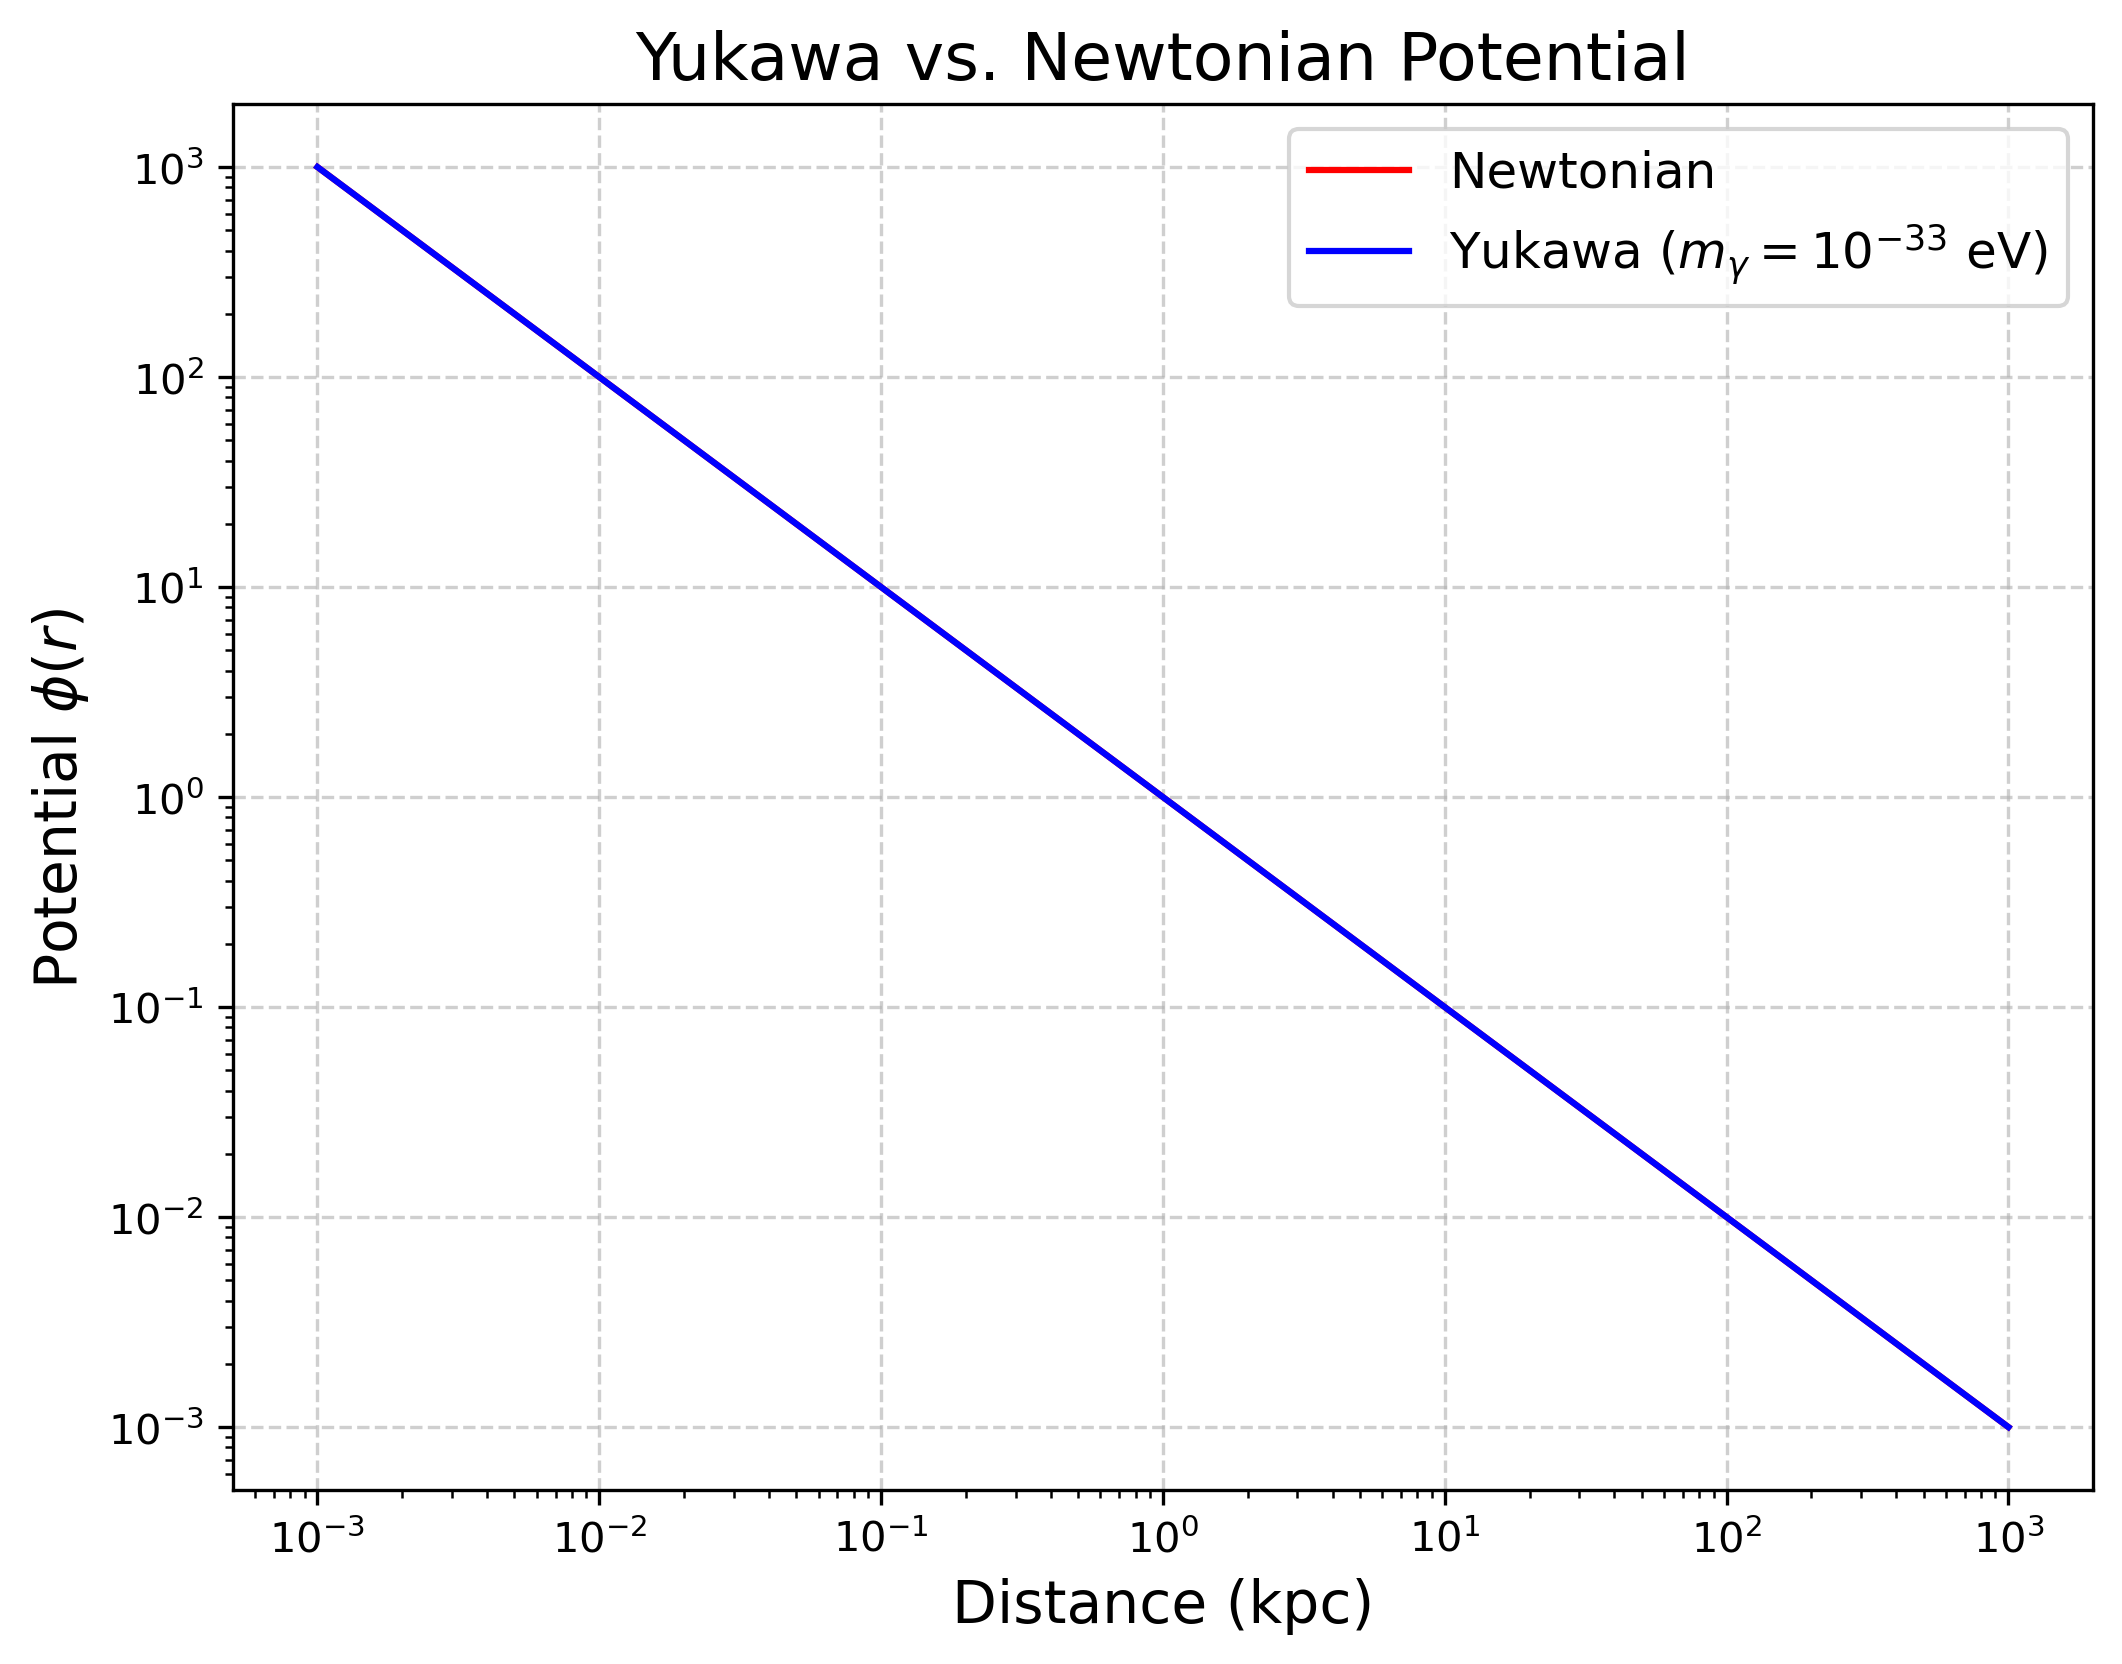
\includegraphics[width=0.8\textwidth]{yukawa_vs_newtonian.png}  
\caption{Yukawa potential (blue) vs. Newtonian (red) for \( m_\gamma = 10^{-33} \, \text{eV} \). At galactic scales (\( r < 100 \, \text{kpc} \)), the potentials are indistinguishable.}  
\label{fig:yukawa}  
\end{figure}  

\begin{figure}[t]  
\centering  
\includegraphics[width=0.8\textwidth]{lensing_anomaly.png}  
\caption{Predicted JWST lensing anomalies (blue) vs. \(\Lambda\)CDM (red) at \( z > 10 \).}  
\label{fig:lensing_anomaly}  
\end{figure}  
